\section{Auswertung}
\label{sec:Auswertung}
\subsection{Messung der Zeitkonstanten $RC$ über die Entladekurve}
Die Entladekurve des $RC$-Kreises wird mit einem Oszilloskop sichtbar gemacht, wie 
in \autoref{fig:aufgabe a - rechteckspannung} zu sehen ist. Die verwendete Frequenz beträgt $f=5\symup{kHz}$.
Im Folgenden werden Wertepaare \{$f [\symup{Hz}], U [\symup{V}]$\} mithilfe von eingezeichneten Hilfslinien abgelesen
(\autoref{fig:aufgabe a - gitter und hilfslinien}) und tabellarisch aufgeführt (\autoref{tab:aufgabe a}). Es ist zu beachten,
dass die Schrittweite von $t$ nicht gleichmäßig gewählt wird, da sich die Werte mit der gewählten Schrittweite mit
geringerem Fehler ablesen lassen.

\begin{figure}
  \centering
  \includegraphics[height=10cm]{content/Aufgabe a - Rechteckspannung.pdf}
  \caption{Entladekurve des Kondensators mit Vorwiderstand}
  \label{fig:aufgabe a - rechteckspannung}
\end{figure}

\begin{figure}
  \begin{subfigure}{0.48\textwidth}
    \centering
    \includegraphics[height=5cm]{content/Aufgabe a - Gitter.pdf}
    \caption{Entladekurve mit Koordinatensystem}
    \label{fig:aufgabe a - gitter}
  \end{subfigure}
  \hfill
  \begin{subfigure}{0.48\textwidth}
    \centering
    \includegraphics[height=5cm]{content/Aufgabe a - Hilfslinien.pdf}
    \caption{Entladekurve mit Hilfslinien}
    \label{fig:aufgabe a - hilfslinien}
  \end{subfigure}
  \caption{Entladekurve mit eingezeichnetem Koordinatensystem und Hilfslinien. Die %
    Skalierung wurde vorher durch Messung der Spannung der Rechteckspannung ermittelt.}
  \label{fig:aufgabe a - gitter und hilfslinien}
\end{figure}

\begin{table}
  \centering
  \caption{Darstellung der Messwertpaare, welche aus \autoref{fig:aufgabe a - gitter und hilfslinien} abgelesen wurden.}
  \label{tab:aufgabe a}
  \begin{tabular}{S[table-format=2.0] S[table-format=1.1]}
    \toprule
    {$s$ [$\symup{\mu s}$]} & {$U$ [V]} \\
    \midrule
    0 &  5,0 \\
    6	&  4,2 \\
    10 & 3,8 \\
    16 & 3,3 \\
    20 & 3,0 \\
    26 & 2,6 \\
    30 & 2,3 \\
    36 & 2,0 \\
    40 & 1,8 \\
    46 & 1,6 \\
    50 & 1,4 \\
    56 & 1,2 \\
    60 & 1,1 \\
    \bottomrule
  \end{tabular}
\end{table}

\begin{figure}
  \centering
  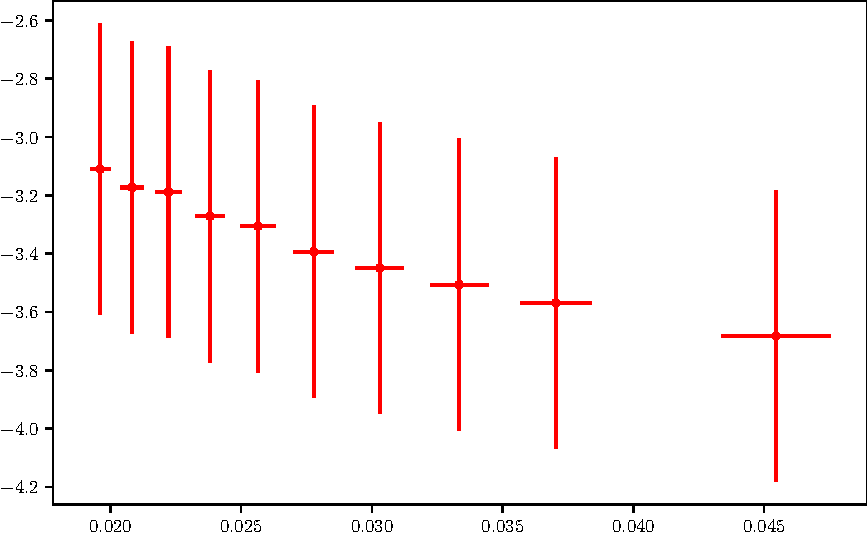
\includegraphics{build/plot_a.pdf}
  \caption{Halblogarithmischer Plot der Wertepaare aus \autoref{tab:aufgabe a} %
  mit Ausgleichsgerade.}
  \label{fig:plot_a}
\end{figure}

Mithilfe der Python-Erweiterungen "numpy" \cite{numpy} und "matplotlib" \cite{matplotlib} werden die Wertepaare der 
\autoref{tab:aufgabe a} halblogarithmisch geplottet und es wird eine Ausgleichsgerade eingezeichnet. Die Parameter der
Ausgleichsgerade vom Typ $ln(U) = m \cdot t + b$ werden zu $m=−0.025050069256648443$ und $b=1.5957959771629942$ bestimmt.
Die Formel des Entladevorgangs eines Kondensators
\begin{equation}
  U_{C} = U_{0}e^{-\frac{1}{RC}\cdot t}
\end{equation}
wird umgestellt zu
\begin{equation}
  ln(U) = ln(U_{0})-\frac{1}{RC}\cdot t
\end{equation}
und entspricht somit der Form der Ausgleichsgerade. Die Zeitkonstante $RC$ ist folglich 
$RC = \frac{1}{m} = 39.920049312222716 \symup{\mu s}$



\subsection{Bestimmung der Zeitkonstante $RC$ über die Frequenabhängigkeit der Amplitude}
Die Spannung am Kondensator $A$ wird ebenso wie die Spannung der Sinusspannungsquelle $U_{0}$ bei variabler
Frequenz $f$ gemessen und tabellarisch in \autoref{tab:aufgabe c} dargestellt. Da sich bei der Messung $U_{0}$
als frequenzunabhängig und zu $U_{0} = 5,2$V bestimmen lässt, ist dieser Wert aus Gründen der
Übersichtlichkeit nicht in der Tabelle aufgeführt. Das Teilungsverhältnis aus $\frac{A}{U_{0}}$ wird berechnet und
gleichermaßen dokumentiert. 

Die Wertepaare \{$f \symup{[Hz]}, \frac{A}{U_{0}}$\} aus \autoref{tab:aufgabe c} werden in ein Diagramm aufgetragen
und es wird eine nicht-lineare Ausgleichsrechnung mit den Python-Erweiterungen "numpy" \cite{numpy} und 
"matplotlib" \cite{matplotlib} durchgeführt. Für den Plot werden nicht die
gerundeten Werte aus \autoref{tab:aufgabe c} verwendet, sondern die exakteren Werte $\frac{A}{U_{0}}$.

\begin{table}
  \centering
  \caption{Messwertpaare Frequenz $f$ und Amplitude $A$ sowie die Relativamplitude $\frac{A}{U_{0}}$.}
  \label{tab:aufgabe c}
  \begin{tabular}{S[table-format=6.0] S[table-format=1.2] S[table-format=1.3]}
    \toprule
    {$f$ [Hz]} & {$A$ [V]} & {$\frac{A}{U_{0}}$} \\
    \midrule
    50     & 2,8	& 0.538 \\
    100    & 2,65 & 0.510 \\
    150    & 2,6  & 0.500 \\
    200    & 2,6  & 0.500 \\
    500    & 2,6  & 0.500 \\
    1000   & 2,5  & 0.481 \\
    1500   & 2,3  & 0.442 \\
    2000   & 2,05 & 0.394 \\
    3000   & 1,8  & 0.346 \\
    4000   & 1,5  & 0.288 \\
    5000   & 1,1  & 0.212 \\
    10000  & 0,68 & 0.131 \\
    20000  & 0,3  & 0.058 \\
    30000  & 0,22 & 0.042 \\
    50000  & 0,14 & 0.027 \\
    100000 & 0,07 & 0.013 \\
    \bottomrule
  \end{tabular}
\end{table}

\begin{figure}
  \centering
  \includegraphics{build/plot_b.pdf}
  \caption{Plot der Wertepaare aus \autoref{tab:aufgabe c} mit nicht-linearer Ausgleichsfunktion \autoref{eq:ausgleichsfunktion aufgabe c}}
  \label{fig:plot_b}
\end{figure}

Die nicht-lineare Ausgleichsrechnung liefert für die Funktion 
\begin{equation}
  \frac{A}{U_{0}} = \frac{1}{\sqrt{1+f^2\cdot (RC)^2}}
  \label{eq:ausgleichsfunktion aufgabe c}
\end{equation}
den Wert $RC = 431,97\symup{\mu s}$.

% RC_a = -39.920049312222716 [\mu s]
% RC_b = [0.00043197] [s]
% RC_c = [-0.00043362] [s]

\subsection{Bestimmung der Zeitkonstanten $RC$ über die Frequenabhängigkeit der Phasenverschiebung%
 zwischen $U_{\symup{C}}$ und $U_{0}$}
 Neben der Amplitude ist auch die Phase zwischen $U_{\symup{C}}$ und $U_{0}$ abhänging von der Frequenz der Spannungsquelle.
 Der Zusammenhang wird durch die Formel
 \begin{equation}
   \varphi(f) = -\arctan(-f\cdot RC)
   \label{eq:Formel für Phasenverschiebung}
 \end{equation}
 beschrieben. 
Die Phase $\varphi$ wird durch den Zusammenhang
\begin{equation}
  \varphi = \frac{a}{b}\cdot 2\symup{\pi}
\end{equation}
berechnet.

\begin{table}
  \centering
  \caption{Messwert Frequenz $f$, Phasenverschiebung $a$, Periodenlänge $b$. Errechnete Phasenverschiebung $\varphi$.}
  \label{tab:aufgabe d}
  \begin{tabular}{S[table-format=6.0] S[table-format=3.1] S[table-format=5.0] S[table-format=1.3] S[table-format=1.3]}
    \toprule
    {$f$ [Hz]} & {$a$ [$\symup{\mu}$s]} & {$b$ [$\symup{\mu}$s]} & {$\varphi$ [rad]}%
     & {$\varphi$ [$\frac{\symup{\pi}}{\symup{rad}}$]}\\
    \midrule
    50      & 0	  & 20000 & 0.000 & 0.000 \\
    100     & 100 & 10000 & 0.063 & 0.020 \\
    150     &	100 & 6500  & 0.097 & 0.031 \\
    200     &	100 & 5000  & 0.126 & 0.040 \\ 
    500     &	100	& 2000  & 0.314 & 0.100 \\
    1000    &	100 & 1000  & 0.628 & 0.200 \\
    1500    & 55  & 630   & 0.549 & 0.175 \\
    2000    &	50  & 500   & 0.628 & 0.200 \\
    3000    & 44  & 330   & 0.838 & 0.267 \\
    4000    & 40  & 250   & 1.005 & 0.320 \\
    5000    & 36  & 200   & 1.131 & 0.360 \\
    10000   & 22  & 100   & 1.382 & 0.440 \\
    20000   & 12  & 52    & 1.450 & 0.462 \\
    30000   & 8   & 34    & 1.478 & 0.471 \\
    50000   & 4,9 & 20    & 1.539 & 0.490 \\
    100000  &	2,5 & 10    & 1.571 & 0.500 \\
    \bottomrule
  \end{tabular}
\end{table}

\begin{figure}
  \centering
  \includegraphics{build/plot_c.pdf}
  \caption{Plot der Wertepaare aus \autoref{tab:aufgabe d} mit nicht-linearer%
   Ausgleichsfunktion \autoref{eq:Formel für Phasenverschiebung}}
  \label{fig:plot_c}
\end{figure}

Auch hier wird für die Wertepaare \{$f \symup{[Hz]}, \varphi$ [rad]\} eine nicht-lineare Ausgleichsrechnung unter 
der Funktion für die Phasenverschiebung (\autoref{eq:Formel für Phasenverschiebung}) durchgeführt. Die Zeitkonstante $RC$ lässt sich
hier zu $RC = 433,62\symup{\mu s}$ bestimmen.

Darüber hinaus wird die frequenzabhängige Amplitude$A$ aus \autoref{tab:aufgabe c} in Abhängigkeit zu der
ebenfalls frequenzabhängigen Phase $\varphi$ aus \autoref{tab:aufgabe d} gesetzt und in einem Polarplot \autoref{fig:plot_d}
visualisiert. Außerdem wird die Funktion 
\begin{equation}
  A(\varphi) = \cos (\varphi) \cdot U_{0}
\end{equation}
zur besseren Interpretation der Messwerte ebenfalls auf den Plot aufgetragen.

\begin{figure}
  \centering
  \includegraphics{build/plot_d.pdf}
  \caption{Hallo}
  \label{fig:plot_d}
\end{figure}

\subsection{Nutzung des RC-Kreises zur Integration von Spannungen hoher Frequenz}
Aus (REFERENZ ZU THEORIE INTEGRATION EINFÜGEN) wird klar, dass ein $RC$-Kreis Spannungen für eine Frequenz $f >> \frac{1}{RC}$
integriert. Als Erstes wird eine Rechteckspannung angelegt. Der Spannungsverlauf einer Rechteckspannung ist jeweils für ein
Zeitintevall konstant, somit ist eine Stammfunktion dazu von linearer Art, wie auch in \autoref{fig:aufgabe d - rechteckspannung}
zu sehen ist.

\begin{figure}
  \centering
  \includegraphics[height=10cm]{content/Aufgabe d - Rechteckspannung.pdf}
  \caption{Rechteckspannung $U_{0}$ und Kondensatorspannung mit $f=5$kHz}
  \label{fig:aufgabe d - rechteckspannung}
\end{figure}

Für eine angelegte Dreieckspannung wird erwartet, dass sich für die Spannung $U_{\symup{C}}$ ein quadratischer Verlauf ergibt,
da eine Dreieckspannung für ein Zeitintevall linear steigt oder sinkt. Dies lässt sich auch in \autoref{fig:aufgabe d - dreieckspannung}
erkennen.

\begin{figure}
  \centering
  \includegraphics[height=10cm]{content/Aufgabe d - Dreieckspannung.pdf}
  \caption{Dreieckspannung $U_{0}$ und Kondensatorspannung mit $f=5$kHz}
  \label{fig:aufgabe d - dreieckspannung}
\end{figure}

Als letztes wird eine Sinusspannungsquelle verwendet. Die Spannung $U_{\symup{C}}$ stellt sich als phasenverschoben
und amplitudenreduziert gegenüber der Spannung $U_{0}$ ein (\autoref{fig:aufgabe d - sinusspannung}). Da eine
Stammfunktion zu der Funktion $f(\omega)=sin(\omega t)$ die Funktion $F(\omega) = \frac{1}{\omega}cos(\omega t)$ ist,
zeigt sich auch hier, dass der $RC$-Kreis für bestimmte Frequenzen als Integrator dienen kann.

\begin{figure}
  \centering
  \includegraphics[height=10cm]{content/Aufgabe d - Sinusspannung.pdf}
  \caption{Sinusspannung $U_{0}$ und Kondensatorspannung mit $f=5$kHz}
  \label{fig:aufgabe d - sinusspannung}
\end{figure}

